
\documentclass[10pt]{article} 
\usepackage[utf8]{inputenc} 
\usepackage[margin=1in]{geometry} 
%\usepackage{pgfplots,wrapfig}
\usepackage{placeins}
\geometry{a4paper} 
\usepackage{multirow}
%\usepackage{caption}
\usepackage{graphicx}
%\usepackage{subcaption}
\usepackage{amsmath}
%\usepackage{booktabs}
%\usepackage{adjustbox}
\usepackage{multicol}
\usepackage{tikz}
\usepackage{subcaption}
\usepackage{graphicx}
\usepackage{pgfplots}
\usepackage{wrapfig}
\usepackage{amsmath,amssymb}

\usepackage{algorithmic}
\usepackage[boxruled, linesnumbered]{algorithm2e}

\usepackage{amsmath}
\newcommand\inlineeqno{\stepcounter{equation}\ (\theequation)}

\vspace{0cm}
\setlength{\parindent}{0cm}
\setlength{\parindent}{1em}
\title{ 
	Probabilistic reasoning and learning project repor:  \protect\\ Play Atari games using artificial neural networks \protect\\  \large a.a. 2017-2018}
\author{ Jary Pomponi}
\date{\vspace{-5ex}}

\newenvironment{Figure}
{\par\medskip\noindent\minipage{\linewidth}}
{\endminipage\par\medskip}
\newcommand{\expect}{\mathop{\mathbb{E}}\nolimits}

\begin{document}
	\maketitle
\begin{multicols}{2}
\section{Introduction}
Reinforcement learning is the area of machine learning that focus in how agents take action in an environment in order to maximize a value called reward by taking. Those agents should learn which action is batter in each situation. In this project I have implement different methods to teach and agent how to play Atari games just by observing just the video and knowing the number of possible actions. In particular the game used is Pong. 

\section{Q learning}

The agents act in an environment, which is formulated as a Markov decision, defined as $(S, A, R, P, \gamma)$ process in which:
\begin{itemize}
	\item $S$ 	is the set of possible states
	\item $A$ is the set of possible actions
	\item $P(s, a, s')$ is the probability of transition from state $s$ to state $s'$ taking action $a$
	\item $R(s, a, s')$ is the immediate reward obtained after transition from $s$ to $s'$ with action $a$
	\item $\gamma$ is the discount factor (how much the future rewards are important)
\end{itemize}

At time step 0 the agent is in the initial state $s_0$ with a given probability. Then the agent pick an action $a_t$, get the reward $r_t$ and transition to next state $s_{t+1}$. This is done until the terminal state is reached. But how the action $a_t$ should be chosen? To chose the best action in each state a function $\pi$, called policy function, is used to specify which action take in each state. The optimal policy $\pi^*$ is the one that maximize the cumulative reward over time. The optimal policy is the one that maximize the expected cumulative reward $\sum_{t\ge0} \gamma^tr_t | \pi$. 

To estimate how good is a policy I will use: 
\[
Q^\pi(s, a) =\expect(\sum_{t\ge0} \gamma^tr_t|s_0 = s, a_0 = a, \pi )
\]
So the optimal policy is the one that maximize the expected total reward.  If the optimal state-action values for the next time step is know then the optimal strategy is to take the action that maximize the expect value of $r + \gamma Q^*(s', a')$. So: 
%\[
%Q^\pi(s, a) =r+ \max_{a'} \gamma Q^* (s', a')|s, a \quad \inlineeqno
%\]
\[
Q^\pi(s, a)=\\
\]
\[ \left\{
\begin{array}{ll}
r+ \max_{a'} \gamma Q^* (s', a')|s, a & \quad	  if \: not \: terminal \\
r & \quad otherwise
\end{array}
\right. \inlineeqno
\] 
 If the state $s$ is an ending state we have $Q^\pi(s, a) = r$.
So the optimal policy can be found by iterating over all the possible pairs and compute the best action in each state, but this is not feasible if the state space is not known or if it is huge like in the Atari case. To overcome this problem a function approximator can be used to estimate $Q(s, a)$. I will do this using artificial neural networks.
%In this project i have used a Reinforcement learning technique called Q learning to see if an agent  

\section{Deep Q-learning (DQN)}
The basic architecture that I have used consists can be seen in Figure 1,a. The networks evaluate each action every time a predict is called but the output is multiplied by a mask in the train process, indicating which action should be taken with a 1 on it and 0s in others.

The problem is threaten as a supervised learning one and the used loss is the so called squared error.: 
\[
L(\Theta_i) = ((r + \gamma Q^*(s', a';\Theta_{i-i})- Q^*(s, a;\Theta_{i} ))^2
\]
This is good because when a larger error shown up the network try to minimize it, but doing this the weights change radically and with those also the target value. To overcome this problem and improve stability and convergence it is useful to clip rewards in -1 and 1 and use another loss called Huber, that loss use two different calculation for large and small error and is defined as: 
\[
 L(\Theta_i)=\left\{
 \begin{array}{ll}
 \frac{1}{2}e^2  & \quad	  if \:|e| < 1 \\
 |e| - \frac{1}{2} & \quad otherwise
 \end{array}
 \right.
\] 
where $e = r + \gamma Q^*(s', a';\Theta_{i-i})- Q^*(s, a;\Theta_{i} )$. This loss give the same weight to low and high error, improving stability and convergence.  

In the next sub-sections I will present the used architectures and explain the train process after a technique called memory replay. 

The train process is simply and consists in agent observing states, acting and collecting rewards. Then update the network weights based on the loss function. 

%A state are simply the image shown on the screen while playing and the actions are defined in the game environment. Since I work with games on a simulated tv it is preferable to skip come frames in order to speed training avoiding not useful information, since many frames will be very similar. Each state is then converted to and gray scale image and then last 4 frames are staked up and fed into the neural network. This is done because adding temporal information to the agent will result in a better action choice. 
%Moreover it should be taking into account that the networks tend to forgot past states and over-fit on current one while learning how to act. This problem is solved using a memory and a target network.

Each network starts with a two convolutional layers and a fully connected layer, as shown in Figure: 1.
 
\subsection{Experience replay memory}
This approach has a problem: while the networks learn how to act in the current state it also forgot the previous explored states. To overcome this problem the passed states are saved in a ring buffer memory with a fixed length. A passed experience at time $t$ is saved as a tuple $(s_t, a_t, r_t, s_{t+1}, ending)$ where $ending$ indicates if the state is an ending one or not and $s_t$ are the states from $t-3$ to $t$ stacked. A subset of the memory is randomly extracted each time a network is trained. 

Fixing the length of the memory is crucial since a small one can not overcome the memory problem but a huge one will slow the learning process, and make this impossible in the worst case, since will contains too old states not useful in late train process.

This method can be further improved by sampling the train states using a probability distribution. To do that I have implemented the prioritized experience replay memory presented in [CITAZIONE]. The main idea is that some transition are more desirable in the train process if the network can learn more from that. In order to know how much the network can learn from a experience it is saved in the memory with an error:
\[
error = |Q(s,a) - T(s)|
\]
Where $T(s)$ is the estimated reward obtainable from $s$. If the learning process is not started $T(s)$ is simply the immediate reward $r$. Then this error is converted to a probability $p_i= (|error_i|+0.001)^\beta$ where $\beta$ weight how much the higher errors are more important than others. Each time a sample is needed a random number $s$, $0\le s \le \sum_i p_i$ would be picked and the memory would be walked summing the probability of visited experience until the sum exceeds $s$. To do that the memory should be sorted based on the $p_i$ since high experience with high error should be favorite. This is very expensive and another approach using a binary unsorted tree structure where each node contains the sum of its children. When a node is updated the change propagates through all the tree 
%Prioritized replay introduces a bias that changes the distribution uncontrollably, this can be corrected by using importance-sampling (IS) weights $w_i = (NP_i)^{-\beta}$, annealing the $\beta$ linearly to 1, that value should be reached when the train process is near to the end. Those weights are normalized by 	$1/(\max_i w_i)$ and folded into the update of the network. 

\subsection{Double DQN (target network)}
To choose the action $a$ that should be picked in a state $s$ and to estimates the future reward obtainable in the new state the same network is used. This network is like a cat chasing its own tail since the network sets itself its targets and then follow them. This could lead to instability, oscillations or divergences. This problem can be solved by using another network to estimates the future reward. 

This new network is simply a copy of the first one frozen in time, so it won't be update using a train procedure, but after several steps the weights from the first network are copied in the second one. With this improvement the Q function becomes: 
\[
Q(s, a) = r + \gamma \max_{a'} Q'(s', a') 
\]

A drawback is that it substantially slows down the learning process. Any change in the Q function is propagated only after the target network update. The intervals between updated are usually in order of thousands of steps, so this can really slow things down. But this improves the stability so it is worth to use it.

\subsection{Duel DQN (DDQN)}
This architecture are shown in Figure 1,b. Dueling DQN uses a specialized Head in order to separate Q to an A (advantage) stream and a V stream. Adding this type of structure to the network head allows the network to better differentiate actions from one another, and significantly improves the learning. With this network the Q function becomes: 
\[
Q(s, a) = V(s) + (A(s, a) - \frac{1}{N} \sum_{a'}^{N} A(s, a'))
\]

The main improvement of this approach is the faster learning. In DQN the network update the Q values only for the specific actions taken in those states. This results in slower learning as we do not learn the Q values for actions that were not taken yet. Dueling architecture starts learning the state-value even if only a single action has been taken at this state by decoupling the Advantage and the value part of the Q function.

\subsection{Training process}

As environment I have used the ai gym library with some preprocessing. The first one consist in transform the images to gray scale and resize them to $84\times84$. Then should be take into account that the Atari game are designed for TVs, so the update frequency are high and this could lead the experience memory to store too many similar images. To overcome this problem only the 4th image are taken, skipping the three before it. in addition to that a state is a stack of the last previously three states and the current one, giving the agent an overview of what happened before and help it in taking the right decision. This helps the agent to know, for example, the moving direction of the ball.

It is important to explore the state space, even if it is huge, before start to learn how to act in it, otherwise the agent will move randomly since it does not know how the game is structured. To do that I have implemented the following approaches, all used in the same time:
\begin{enumerate}
\item Populate replay memory: the train process starts only when the memory contains a certain amount of experiences
\item No actions taken: at the beginning of the game the agent stay stationary for a random amount of frames from 1 to 30. Those frames are not added to the memory. This helps exploration and train speed, since the starting states are all very similar. 
\item Random action pick: the probability of picking a random action starts from 1.0 and decrease linearly to 0.02 in 1 million of frames. This is the crucial exploration strategy since allow the agent to explore a large amount of states and actions with the associated reward. 
\end{enumerate}

The final algorithm is: 

\begin{algorithm}[H]
\caption{Q-DQN generic algorithm}
\begin{algorithmic} 
\STATE -Initialize memory M to capacity N
\STATE -Initialize action-value function with random weights
\FOR{episode=1 to Eps}
\STATE get preprocessed state $s$
\WHILE{game is not done}
\STATE -with probability $\epsilon$ get a random action otherwise select $a_t=\max_{a'} Q(s, a')$ 
\STATE -perform action, collect reward $r$ and \\ next state $r_n$
\STATE -store experience $(s, a, r, s_n)$ in \\ memory M
\IF {enough experience in M}
\STATE -sample random batch from M and
\STATE update batch targets 
\\ using formula $(1)$
\STATE -update network weights according \\ to loss
\ENDIF
\ENDWHILE
\ENDFOR
\end{algorithmic}
\end{algorithm}

If the memory is a prior one then after the update of the network the tree of probability should be updated. More than that if a target network is being used then after the update the weights should be copied if needed.

\section{Empirical evaluations}

\begin{figure*}
	\centering
	\begin{subfigure}[b]{0.40\textwidth}
	\centering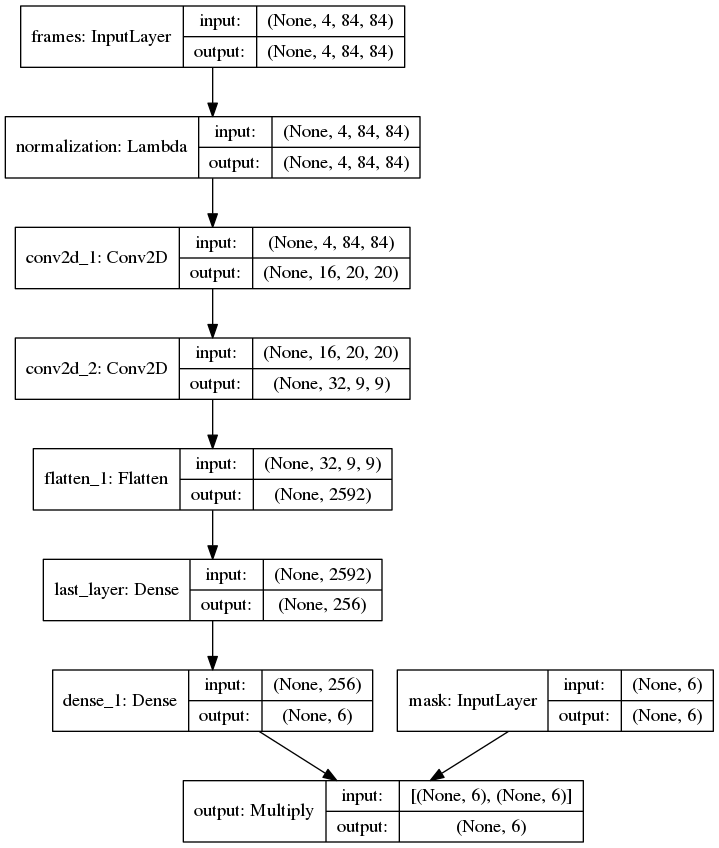
\includegraphics[width=\linewidth]{model.png}
	\captionof{figure}{DQN architecture}
	\end{subfigure}
	%
	\begin{subfigure}[b]{0.59\textwidth}
	\centering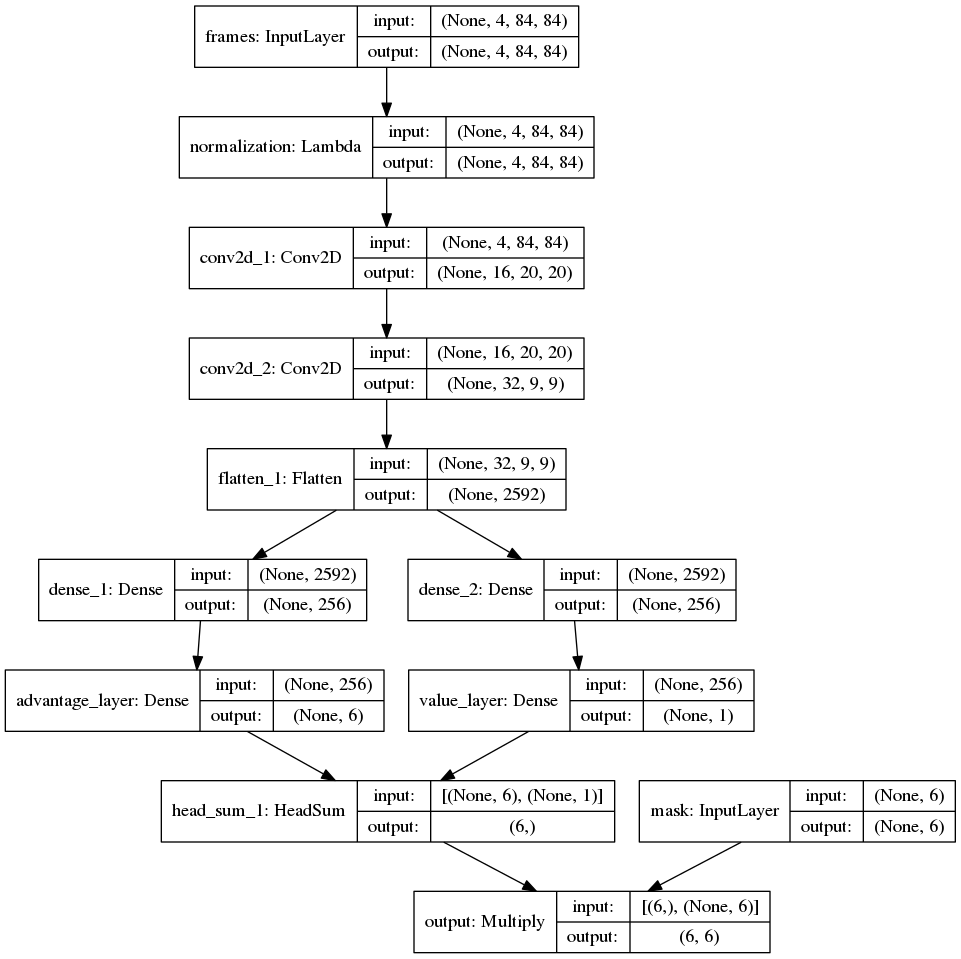
\includegraphics[width=\linewidth]{duel.png}
	\captionof{figure}{Duel DQN architecture}
	\end{subfigure}
	\setcounter{figure}{0}    
	\captionof{figure}{Architecture implemented in this project}
\end{figure*}
\iffalse
\begin{center}
	\centering
	\includegraphics[height=45mm]{../results/rep_attr.png}
	\setcounter{figure}{0}  
	\label{fig}  
	\captionof{figure}{Repulsive and attractive factor varying $\sigma$}
\end{center}
\section{Empirical evaluation and conclusions}
\begin{figure*}
	\centering
	\begin{subfigure}[b]{\textwidth}
		\centering
	\begin{minipage}{.32\linewidth}
		\centering\includegraphics[width=\linewidth]{../results/comm_3.png}
		3 agents.
	\end{minipage}
	\begin{minipage}{.32\linewidth}
		\centering\includegraphics[width=\linewidth]{../results/comm_4.png}
		4 agents.
	\end{minipage}
	\begin{minipage}{.32\linewidth}
		\centering\includegraphics[width=\linewidth]{../results/comm_5.png}
		5 agents.
	\end{minipage}
		\begin{minipage}{.32\linewidth}
			\centering\includegraphics[width=\linewidth]{../results/comm_6.png}
			6 agents.
		\end{minipage}
		\begin{minipage}{.32\linewidth}
			\centering\includegraphics[width=\linewidth]{../results/comm_7.png}
			7 agents.
		\end{minipage}
		\begin{minipage}{.32\linewidth}
			\centering\includegraphics[width=\linewidth]{../results/comm_8.png}
			8 agents.
		\end{minipage}
		%\captionof{figure}{Experiments on communication range varying agents and fires}
	\end{subfigure}
\setcounter{figure}{1}    
\captionof{figure}{Experiments on communication range varying agents and fires}
\end{figure*}

\fi

\end{multicols}
\newpage
\end{document}
